\subsection{Variation of Photon Density with Altitude}
\label{sec:VariationOfPhotonDensity}

To determine the number of photons with increasing altitude, a simulation was ran with several constellations. These constellations differ only on the constellation altitude. Each constellation exists of a single transmitter and receiver, on the same orbit. Furthermore, to reduce errors not due to the altitude effect, the scattering coefficients and elevation remain constant over the entire \ac{DEM} area.

The scattering coefficients values used where 1.5 for the index of refraction, 1.3 for the Minnaert correction and -0.5 for the Henyey-Greenstein correction. The area over which the simulation ran is a rectangle stretching from (48$^\circ$ lat; 8$^\circ$ long) to (54$^\circ$ lat; 9$^\circ$ long). The \ac{laser} (500 nm) that was used has 10W of \ac{laser} power, spread over 5000 pulses per second, each with a length of 1ns. The receiver satellite has an aperture of 8x8 cm (0.0064 m$^2$) with a perfect receiver. The constellation orbital parameters are as follows:

\begin{itemize}
	\item Semi-major axis:	Earth radius + altitude (variable),
	\item Eccentricity: 0,
	\item Inclination: 90$^\circ$,
	\item Right ascension of ascending node: 8.5$^\circ$,
	\item Argument of perigee: 0$^\circ$,
	\item True anomaly: 0$^\circ$.
\end{itemize}1

The results are shown in table \ref{table:simulationHeight} and visualized in figure \ref{fig:simulationHeight}. The datapoints show a clear exponential decaying trend. This trend can be approximated with the mathematical function $y=e^{-0.0052 \cdot x + 0.6558}$. This function shows a high decay rate with increasing altitude. For example moving from altitude of 500km to 350km halves the number of received photons. To compensate for this effect, one would have to design the \ac{laser} to have double the power, or the receiver double the aperture. This is because both of these parameters directly effect the number of received photons. 

\small
\begin{table}[ht!]
\begin{tabular}{| l | c | c | c | c | c | c | c |c | c |}
	\hline
		Altitude [km] &        300 &     325 &      350 &      375 &     400 &     425 &     450 &     475 &      500 \\
	\hline
		Average \# photons &  0.4249 &  0.3613 &   0.2991 &   0.2692 &  0.2483 &  0.2054 &  0.1843 &  0.1641 &   0.1483 \\
	\hline
\end{tabular}
\caption{Simulation results for varying altitude}
\label{table:simulationHeight}
\end{table} 

\begin{figure}[ht!]
	\centering
		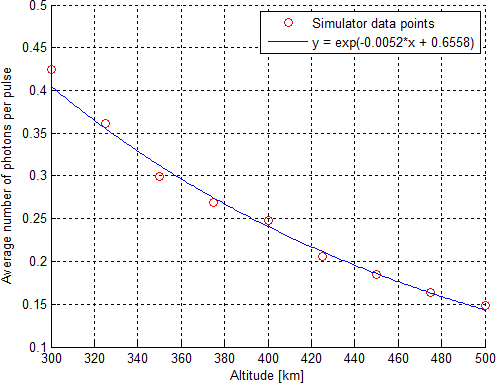
\includegraphics[width=0.8\textwidth]{chapters/img/simulationHeight.png}
	\label{fig:simulationHeight}
	\caption{Height variation effect in the \# received photons}
\end{figure}

From this simulation, one can conclude that purely on the bases of received photons, a lower altitude is better. This is in direct contradiction to the drag analysis. However higher altitudes are possible, with increased \ac{laser} power and/or receiver aperture area.